% Latex template: mahmoud.s.fahmy@students.kasralainy.edu.eg
% For more details: https://www.sharelatex.com/learn/Beamer

\documentclass{beamer}					% Document class

\setbeamertemplate{footline}[text line]{%
  \parbox{\linewidth}{\vspace*{-8pt}Statistical Methods For Stochastic Biological Systems\hfill\insertshortauthor\hfill\insertpagenumber}}
\setbeamertemplate{navigation symbols}{}

\usepackage[english]{babel}				% Set language
\usepackage[utf8x]{inputenc}			% Set encoding

\mode<presentation>						% Set options
{
  \usetheme{default}					% Set theme
  \usecolortheme{default} 				% Set colors
  \usefonttheme{default}  				% Set font theme
  \setbeamertemplate{caption}[numbered]	% Set caption to be numbered
}

% Uncomment this to have the outline at the beginning of each section highlighted.
%\AtBeginSection[]
%{
%  \begin{frame}{Outline}
%    \tableofcontents[currentsection]
%  \end{frame}
%}

\usepackage{graphicx}					% For including figures
\usepackage{booktabs}					% For table rules
\usepackage{hyperref}					% For cross-referencing

\title{Deep generative models for biologists}	% Presentation title
\author{Clayton W. Seitz}								% Presentation author
\date{\today}									% Today's date	

\begin{document}

% Title page
% This page includes the informations defined earlier including title, author/s, affiliation/s and the date
\begin{frame}
  \titlepage
\end{frame}

% Outline
% This page includes the outline (Table of content) of the presentation. All sections and subsections will appear in the outline by default.
\begin{frame}{Outline}
  \tableofcontents
\end{frame}

% The following is the most frequently used slide types in beamer
% The slide structure is as follows:
%
%\begin{frame}{<slide-title>}
%	<content>
%\end{frame}


\section{Generative Models}

\begin{frame}{The logic of generative modeling}

Say we have a set of variables $\mathbf{x} = (x_{1},x_{2},...,x_{n})$ which might have some statistical dependence\\
\vspace{0.1in}
The variable $\mathbf{x}$ might be an amino acid sequence, gene expression data, microscopy image, etc.\\
\vspace{0.1in}
\begin{itemize}
\item Often we are handed a batch of empirical samples $\{\mathbf{x}_{i}\}_{i=1}^{N}$
\item We want to know the generating distribution $p(\mathbf{x})$
\end{itemize}

In supervised \textcolor{red}{generative learning}, we try to explicity learn the joint distribution $p(\mathbf{x}) = \prod_{i=1}^{N-1}p(x_{i}|x_{i+1:N})p(x_{N})$, which is generally more difficult than discriminative learning. 

\end{frame}

\begin{frame}{Applying deep generative models to biological data}
\begin{figure}
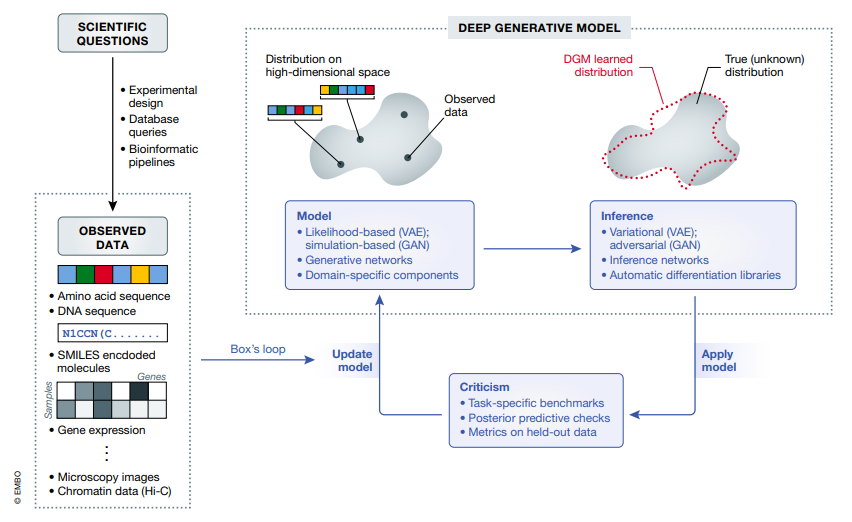
\includegraphics[height=65mm, width=105mm]{dbm}
\end{figure}
\end{frame}

\begin{frame}{Perks of generative modeling}

\begin{itemize}
\item Fitting complete multivariate distributions $p(\mathbf{x})$ goes beyond correlation-based or clustering approaches
\item Correlations cannot discover partial correlation in the context of other neighbors
\item Fitting $p(\mathbf{x})$ permits sampling based inference
\end{itemize}

\end{frame}

\begin{frame}{Generative learning: probabilistic graphical models}

PGMs may aid in the discovery of gene networks that drive complex diseases  

\begin{center}
\begin{figure}
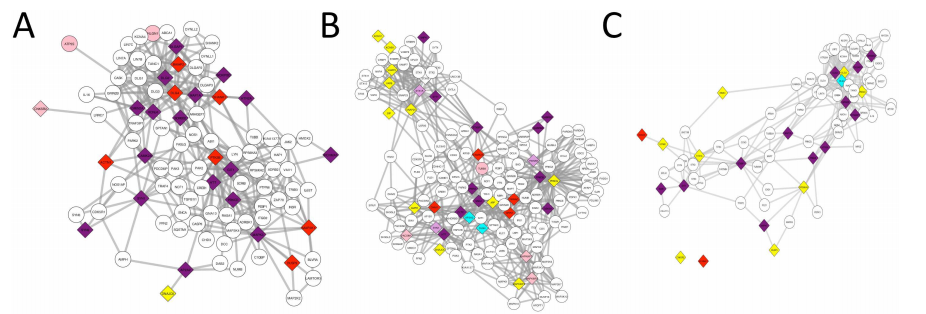
\includegraphics[width=1.0\textwidth]{gene-net}
\caption{\textbf{Bayesian networks} for gene network discovery in (A) Schizophrenia (B) Epilepsy (C) Autism. Taken from Mezlini et al. 2017}
\end{figure}
\end{center}

\end{frame}

\begin{frame}{Probabilistic graphical models (PGMs) are generative}

\begin{center}
\begin{figure}
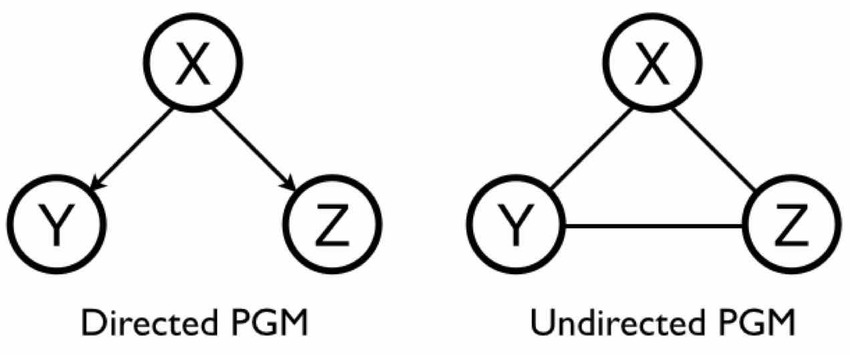
\includegraphics[width=0.75\textwidth]{pgm}
\caption{\textbf{PGMs} for the joint distribution $P(X,Y,Z)$}
\end{figure}
\end{center}

Two important classes are directed PGMs (\textcolor{red}{Bayesian networks}) and undirected PGMs (\textcolor{red}{Markov random fields}). Many applications: image processing, genomics, statistical mechanics

\end{frame}


\begin{frame}{Generative learning: variational autoencoder (VAE)}

\begin{center}
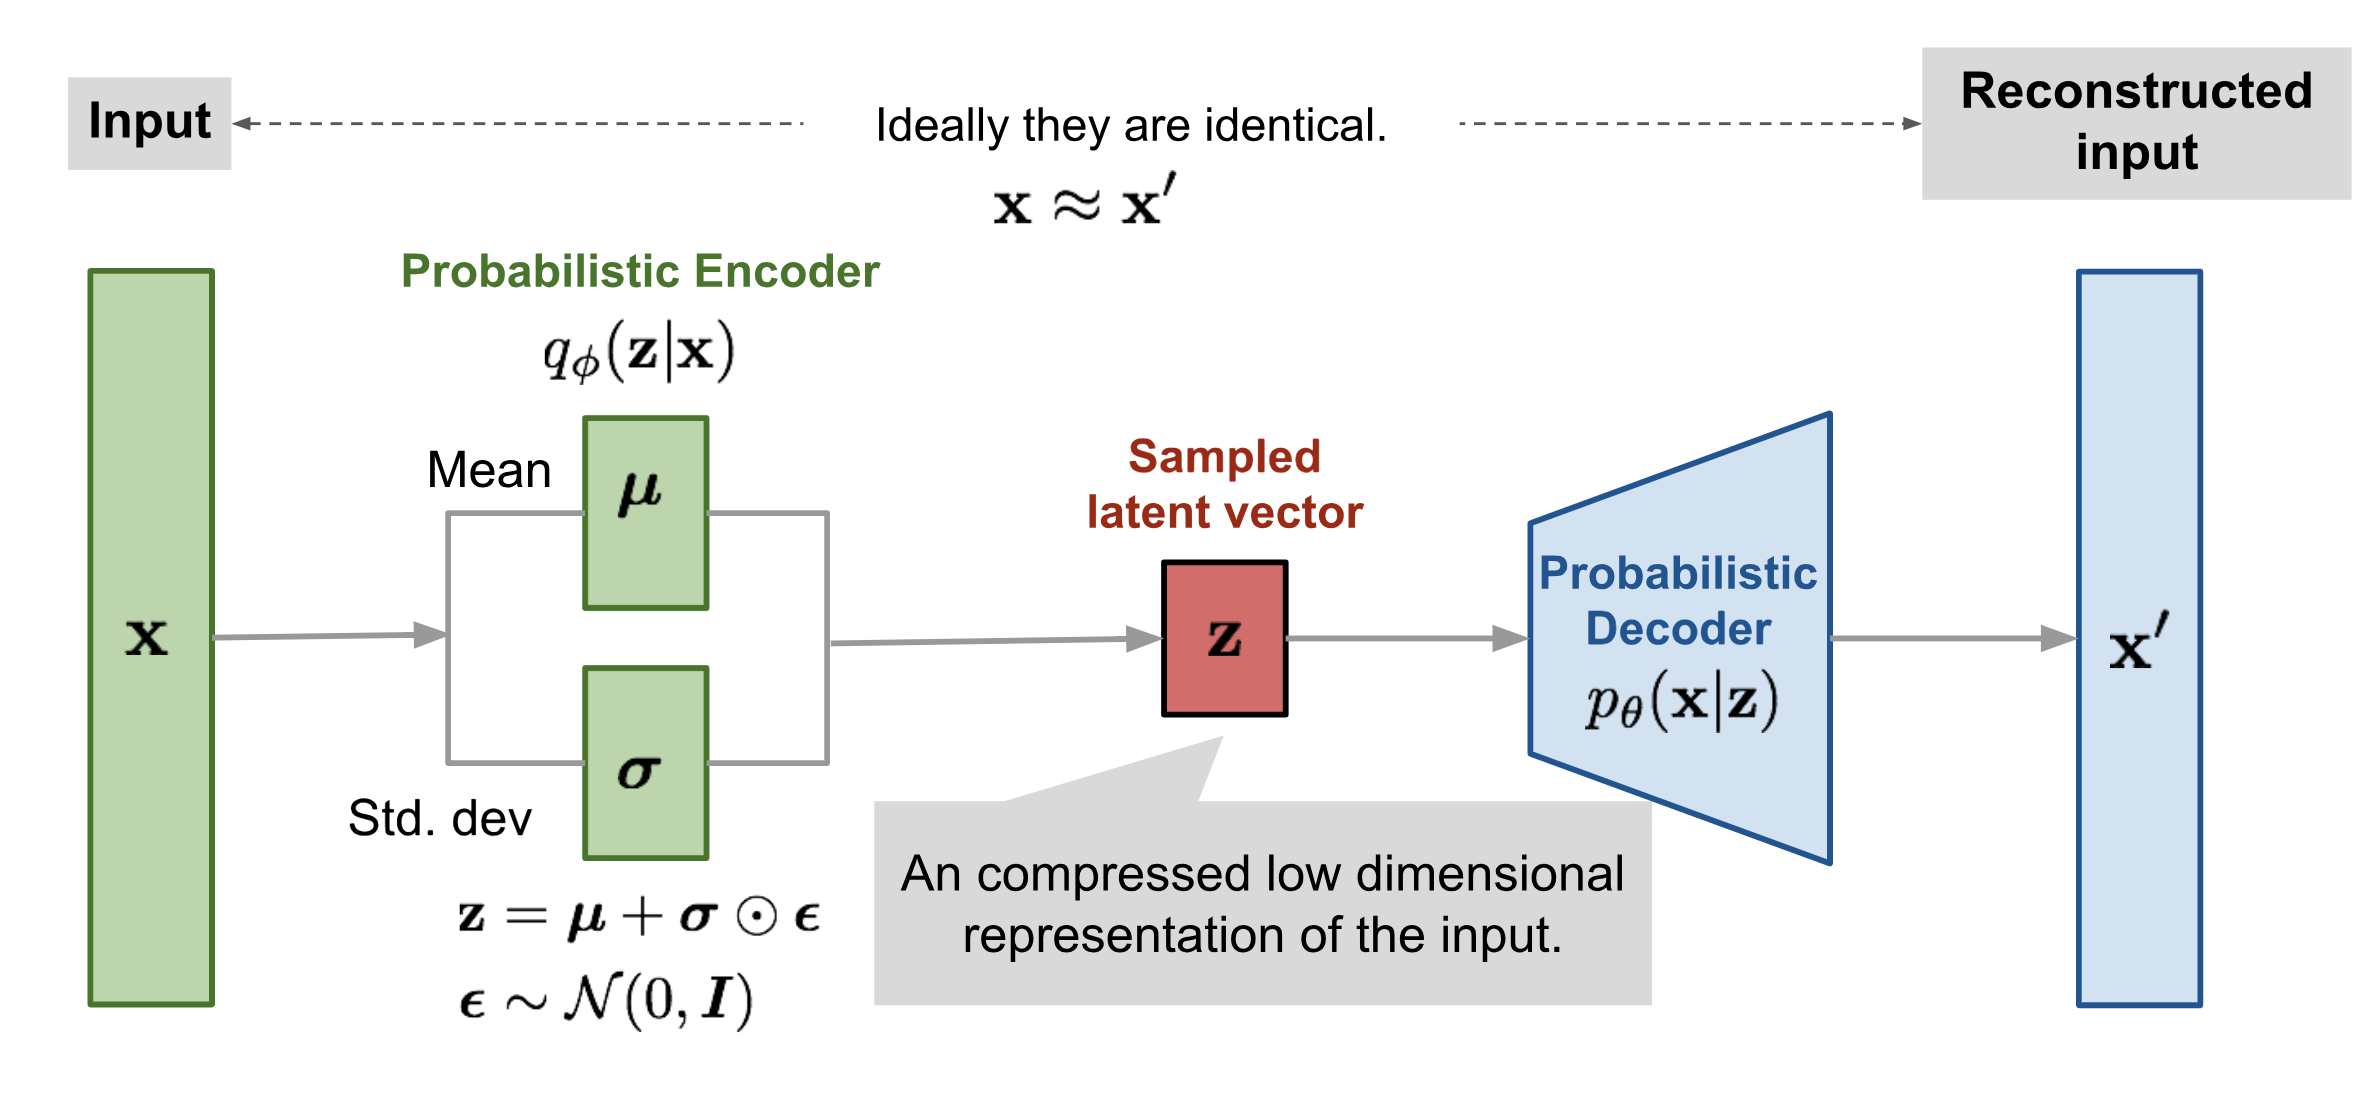
\includegraphics[width=1.0\textwidth]{vae}
\end{center}

\end{frame}

\begin{frame}{Embedding the latent space of a VAE in 2D}

\begin{figure}
\begin{center}
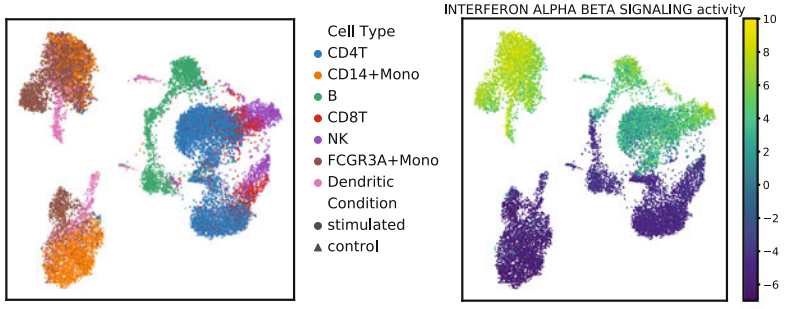
\includegraphics[width=1.0\textwidth]{immune}
\end{center}
\caption{Phenotype segregation using a VAE on single-cell transcriptomics data. Taken from Seninge et al.}
\end{figure}

\end{frame}

\begin{frame}
\begin{columns}
\begin{column}{0.5\textwidth}
\textbf{Probabilistic graphical model}s\\
\vspace{0.1in}
\textcolor{green}{+} structured representation\\
\vspace{0.1in}
\textcolor{green}{+} rigidity = efficiency\\
\vspace{0.1in}
\textcolor{red}{-} rigid assumptions may not fit\\
\vspace{0.1in}
\textcolor{red}{-} feature engineering
\end{column}
\begin{column}{0.5\textwidth}  %%<--- here
\begin{center}
\textbf{Deep learning}\\
\vspace{0.1in}
\textcolor{red}{-} Neural net "goo"\\
\vspace{0.1in}
\textcolor{red}{-} Difficult parameterization\\
\vspace{0.1in}
\textcolor{green}{+} Flexible, high capacity\\
\vspace{0.1in}
\textcolor{green}{+} Feature learning\\
\vspace{0.1in}
\end{center}
\end{column}
\end{columns}
\end{frame}

\begin{frame}{The sampling problem}

We also may not know the proper normalization constant or \textcolor{red}{partition function} $Z$. Say we have

\begin{equation*}
p(\mathbf{x}) = \frac{1}{Z}\tilde{p}(\mathbf{x})
\end{equation*}

where $p(\mathbf{x})$ is easy to compute but $Z$ is (too) hard to compute.\\
\vspace{0.1in}
This \textcolor{red}{very important} situation arises in several contexts:\\
\vspace{0.1in}
1. In \textcolor{red}{Bayesian models} where $p(x_{1},x_{2}) := p(x_{1}|x_{2})p(x_{2})$ is easy to compute but
$Z = \int p(x_{1}|x_{2})p(x_{2})dx_{2}$ can be very difficult or impossible to
compute.\\
\vspace{0.1in}
2. In models from statistical physics, e.g. the Ising model, we only know
$\tilde{p}(\mathbf{x}) = e^{−H(\mathbf{x})}$ where $H(\mathbf{x})$ is the Hamiltonian

\end{frame}


\section{References}

% Adding the option 'allowframebreaks' allows the contents of the slide to be expanded in more than one slide.
\begin{frame}[allowframebreaks]{References}
	\tiny\bibliography{references}
	\bibliographystyle{apalike}
\end{frame}

\end{document}